\documentclass[10pt, a4paper]{beamer}
\usepackage{array}
\usepackage{graphicx}
\graphicspath{ {images/} }
\usetheme{Berkeley}
\usecolortheme{sidebartab}

\begin{document}
	\setbeamertemplate{sidebar left}{}
	\title{Progress Presentation-I}
	\subtitle{e-Yantra Summer Internship-2016 \\ \vspace{2mm}Exploring WICED Sense }
	\author{Chinmay Patil\\Imran Khan\\ \vspace{5mm}
	Mentor: Santosh , Uttam }
	\institute{IIT Bombay}
	\date{\today}
	
	\frame{\titlepage}

\setbeamertemplate{sidebar left}[sidebar theme]
\section{Overview of Project}
\begin{frame}{Overview of Project}
	\begin{itemize}
		\item Project Title : Exploring WICED Sense
		\item Objective : To develop applications for Wiced Sense Tag and make a user friendly system which can be used in real world.
		\item Deliverables : \begin{enumerate}
		      \item Code to acquire data from wiced sense tag on local machine.
		      \item Procedure for pushing the real time sensor data from wiced sense into database.
		      \item Develop an effective algorithm for area mapping using Firebird V and wiced sense.
		      \item Systematic documentation of developed codes and design procedures.
		\end{enumerate}
	\end{itemize}
\end{frame}

\setbeamertemplate{sidebar left}[sidebar theme]
\section{Introduction}
\begin{frame}{Introduction}
  \caption \textbf {WICED SENSE TAG}
  \centering
  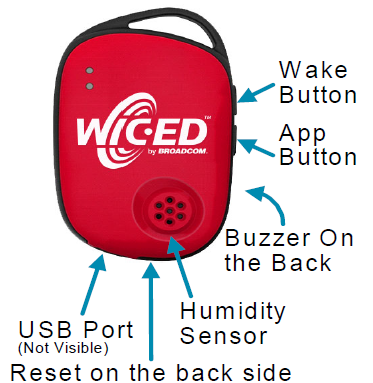
\includegraphics[width=3cm, height=4cm]{broadcom-wiced-sense.png}
  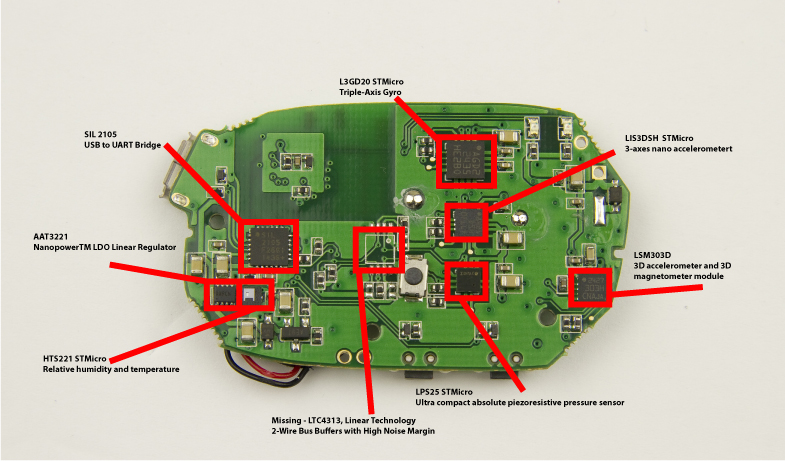
\includegraphics[scale=0.3]{PCBLayoutFront.jpg}
  \end{frame}

\setbeamertemplate{sidebar left}[sidebar theme]
\section{Introduction}
\begin{frame}{Introduction}
  \textbf{What is BLE ? How is it different from other communication technologies ?}
  \begin{itemize}
  \item Bluetooth 4.0 / Bluetooth Low Energy / Bluetooth Smart
  \item Lowest possible power consumption
  \item Specifically optimized for low cost
  \item Low complexity
  \item Low Latency
  \item Wide Interoperability Infrastructure
  \end{itemize}
\end{frame}

\setbeamertemplate{sidebar left}[sidebar theme]
\section{Overview of Task}
\begin{frame}{Overview of Task}	

\begin{center}
\begin{tabular}{ | m{0.5cm}| m{5cm} | m{1.5cm}| } 
\hline
Sr. &  Task
& Deadline\\ 
\hline
1. & Download the SDK for WICED Sense, and get familiar with it & 4 Days  \\ 
\hline
2. & Go through different videos/documents related to WICED Sense and
Display the WICED Sense data on the Desktop
& 4 Days \\
\hline
3. & Fetch the obtained data in the desktop to the online database & 4 days\\

\hline
\end{tabular}
\end{center}
\end{frame}

\begin{frame}{Overview of Tasks}
\begin{center}
\begin{tabular}{ | m{0.5cm}| m{5cm} | m{1.5cm}| } 
\hline
Sr. & Task
& Deadline\\ 
\hline
4. & Develop a notification system making use of the fetched values
Eg: 1) If the temperature of the room falls below say 30֯ C, notify the user
      2) If speed of the object crosses a specified threshold  value,                               the object should stop. Can be done with Firebird V for testing & 6 Days\\	
\hline
5. & Using the sensor values, develop an effective algorithm for mapping of Firebird V robot inside specific area & 10 Days\\
\hline
6. & Implementation and calibration & 7 Days\\
\hline
7. & Design Tutorial and systematic Documentation of project. & 3 Days\\
\hline
\end{tabular} 
\end{center}
\end{frame}

\section{Task Accomplised}
\begin{frame}{Task Accomplised}
	\begin{itemize}
	   \item Downloading the SDK for WICEDSense, and getting familiar with it.\\
	   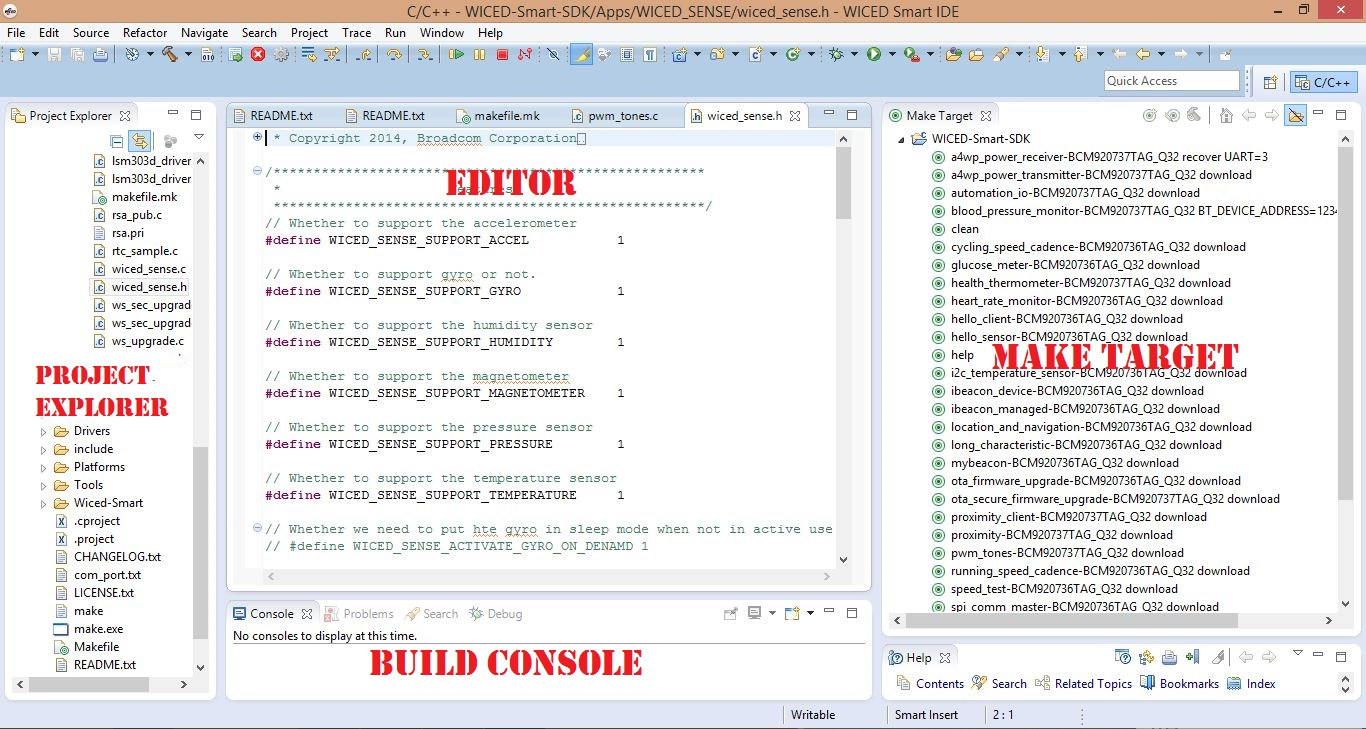
\includegraphics[scale=0.2]{Wiced-sdk.JPG}
	\end{itemize}
\end{frame}

\section{Task Accomplised}
\begin{frame}{Task Accomplised}
	
	
	   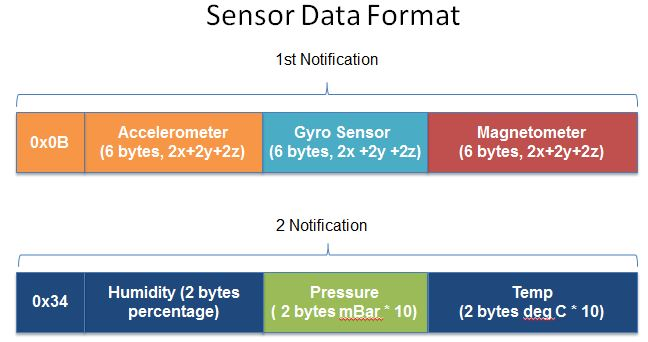
\includegraphics[width=5cm, height=4cm]{PacketFormat.JPG}
	   \vspace{3mm}
	   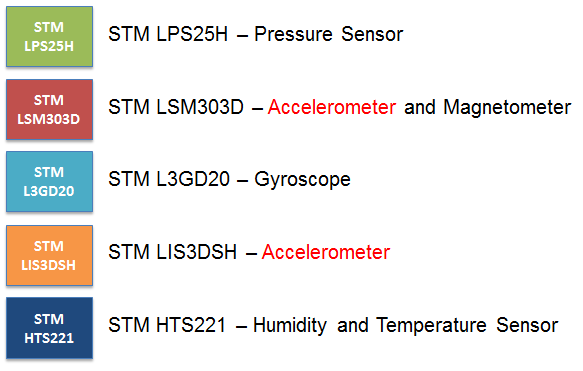
\includegraphics[width=5cm, height=4cm]{Sensors.png}
	
\end{frame}

\section{Task Accomplished}
\begin{frame}{Task Accomplished}
	\begin{itemize}
	   \item Connecting Wiced-Sense to the system and getting the device data. \\
	
	   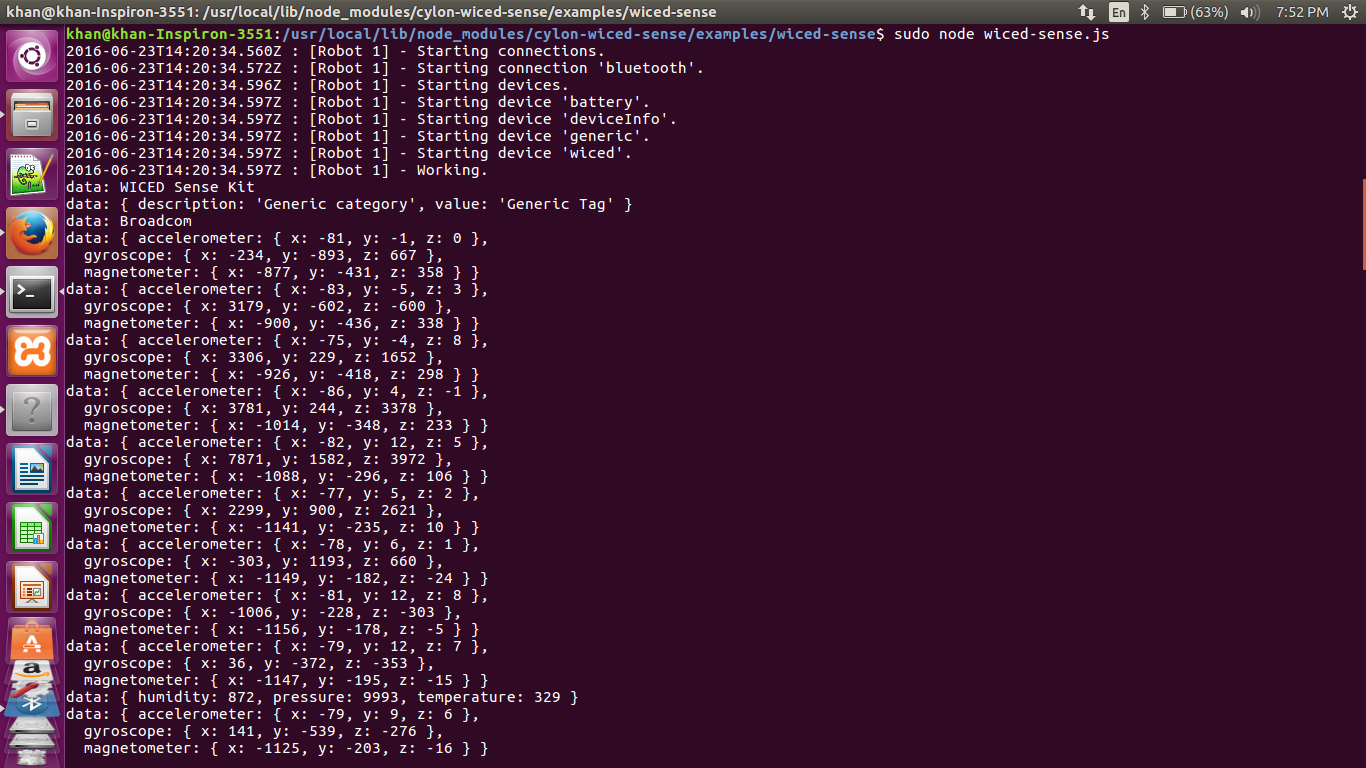
\includegraphics[width=7cm, height=4cm]{ble-data.png}
	\end{itemize}
\end{frame}

\section{Task Accomplished}
\begin{frame}{Task Accomplished}
	\begin{itemize}
	  \item Converted the data into CSV format so that it can be easily extracted and inserted into mySQL database.  \\
	  
	  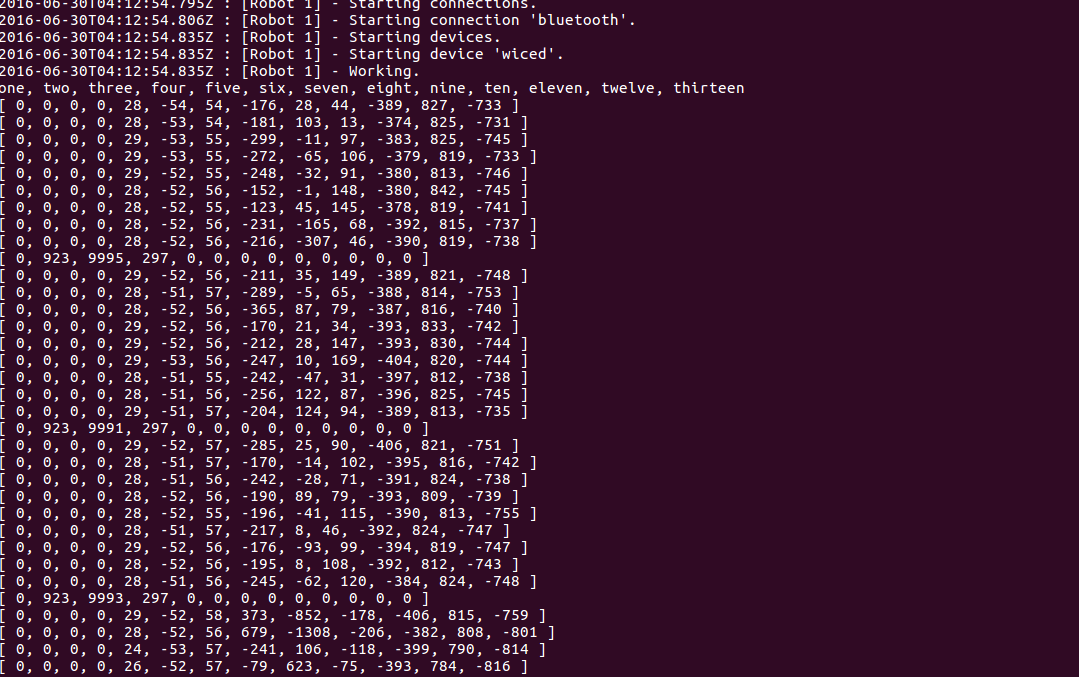
\includegraphics[width=7cm, height=4cm]{csvformat.png}
	\end{itemize}
\end{frame}

\section{Task Accomplished}
\begin{frame}{Task Accomplished}
	\begin{itemize}
	  \item Data from the terminal is logged into csv file on the local system. \\
	  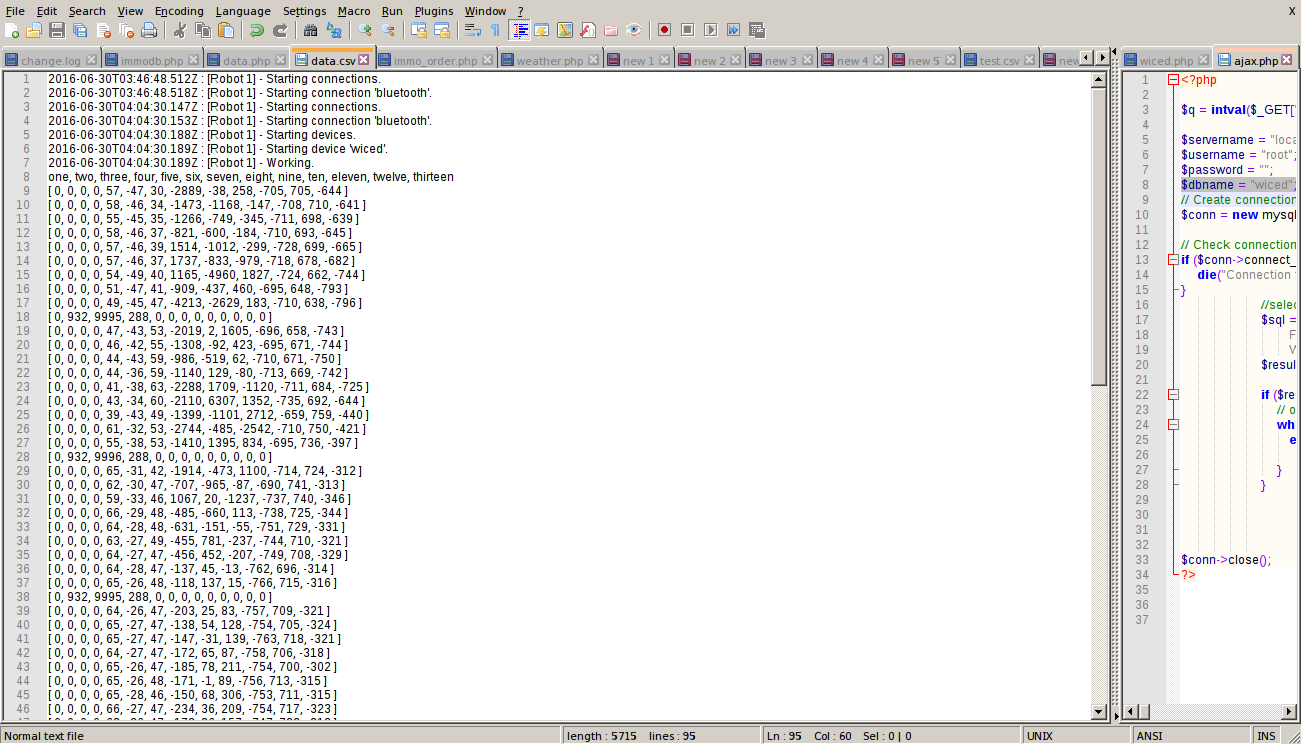
\includegraphics[width=7cm, height=4cm]{notepaddatacsv.png}
	\end{itemize}
\end{frame}

\section{Task Accomplished}
\begin{frame}{Task Accomplished}
	\begin{itemize}
	  \item  Pushed the data from local system to mySQL database.\\
	  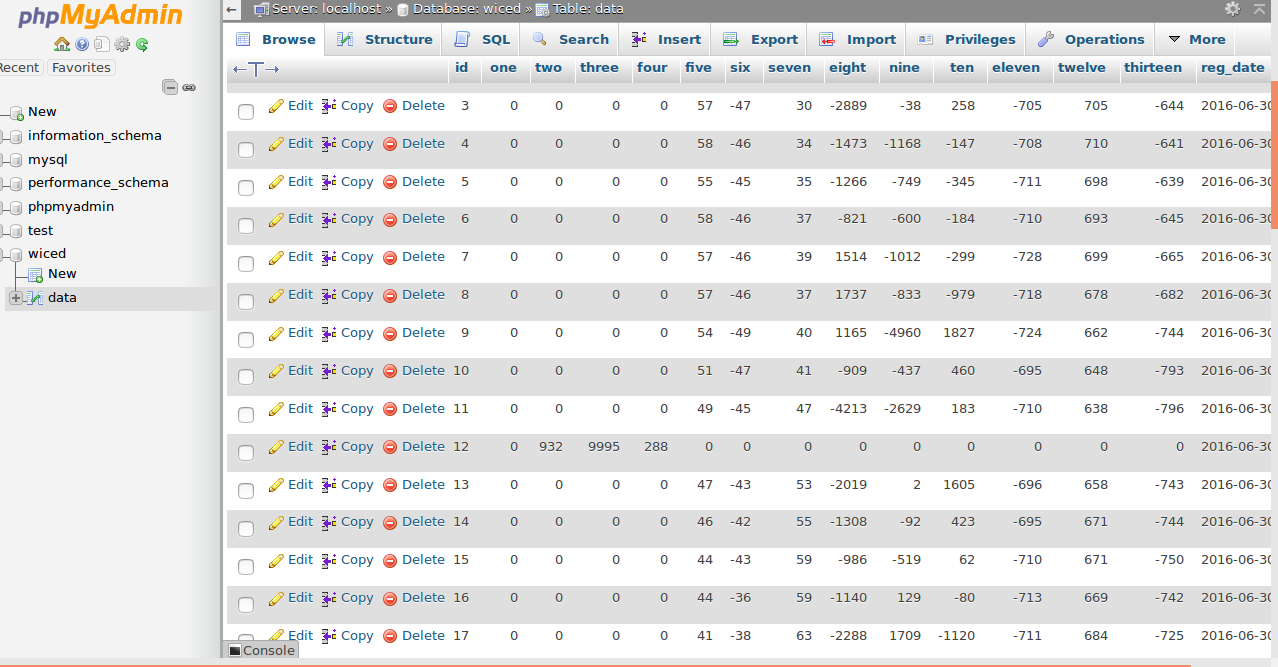
\includegraphics[width=7cm, height=4cm]{database.png}
	\end{itemize}
\end{frame}

\section{Task Accomplished}
\begin{frame}{Task Accomplished}
	\begin{itemize}
	  \item All the sensors data are fetched from the database and dynamically displayed on the webpage.\\
	\end{itemize}
\end{frame}

\section{Working on..}
\begin{frame}{Working on..}
	\begin{itemize}
	  \item Plotting graph/charts to display real time sensor data.
	  \item Making GUI for different applications.
	\end{itemize}
\end{frame}

\section{Challenges Faced}
\begin{frame}{Challenges Faced}
	\begin{itemize}
		\item Installing Cylon js , Cylon-ble , Cylon-wiced-sense and all the other packages in ubuntu so that we acquire data from Wiced sense tag.
		\item Recovering firmware on wiced sense tag using wiced sdk.
		\item Pushing the data from local system to mySQL database.
	\end{itemize}
\end{frame}

\section{Future Plans}
\begin{frame}{Future Plans}
	\begin{itemize}
		\item To develop a notification system which will alert the user of a particular event.
		\item To develop an effective algorithm for mapping of Firebird V robot using the sensor data from wiced sense.
	\end{itemize}
\end{frame}

\section{References}
\begin{frame}{References}
	\begin{itemize}
		\item https://cylonjs.com/documentation/platforms/wiced-sense/
		\item https://www.bluetooth.com/what-is-bluetooth-technology/bluetooth-technology-basics/low-energy
		\item http://stackoverflow.com/questions/tagged/javascript
	\end{itemize}
\end{frame}

\section{Thank You}
\begin{frame}{Thank You}
	\centering THANK YOU !!!
\end{frame}
\end{document}
